\documentclass[11pt]{article}
%\usepackage{url}
%\usepackage{algorithmic}
\usepackage[margin=1in]{geometry}
\usepackage{datetime}
\usepackage[margin=2em, font=footnotesize]{caption}
\usepackage{graphicx}
\usepackage{mathpazo} % use palatino
\usepackage[scaled]{helvet} % helvetica
\usepackage{microtype}
\usepackage{amsmath}
\usepackage{subfigure}
\usepackage{listings}
\usepackage{wrapfig}
\usepackage{ amssymb }
% Letterspacing macros
\newcommand{\spacecaps}[1]{\textls[200]{\MakeUppercase{#1}}}
\newcommand{\spacesc}[1]{\textls[50]{\textsc{\MakeLowercase{#1}}}}
\lstdefinestyle{myCustomMatlabStyle}{
  language=Python,
  stepnumber=1,
  numbersep=10pt,
  tabsize=4,
  showspaces=false,
  showstringspaces=false
}
\lstset{basicstyle=\footnotesize,style=myCustomMatlabStyle}
\title{Summer report - Motility as a driver for microbial cross-feeding }
\date{September\\2021}
\author{Kelvin Leung, Shavindra Jayasekera}
\usepackage{dsfont}
\usepackage{varwidth}
\usepackage{float}
\usepackage{bm}
\usepackage{mathtools}

\begin{document}
\maketitle
\section{Introduction}
Microbes are known to produce compounds that can be costly to themselves but beneficial to their surrounding cells and this has led to research \cite{oliveira} into models which examined the cooperation between microbial strains and species where the microbes make multiple secretions which can be exchanged among themselves. However, the system only considered the impact from the reproduction processes of the microbes and haven't taken into account the impact of the cells moving. \\
However, it has also been shown in \cite{rps}\cite{wakano} that in spatial ecoevolutionary models, motility of the cells involved can play an important role to the survival and reproduction of the microbes. With different motility, the same system can have vastly different stable states in long time.\\\\
In this project, we have therefore investigated the effect motility plays in the evolution of a two-public-goods systems using a stochastic lattice model where cells are allowed to move as well as other normal functions, e.g. reproduction, selection etc..\\
The aim is to investigate how cross-feeding will be affected in this model, i.e. will motility increase the surviving chances of inter-cooperating microbes which are dependent on the secretion of the other species, and have lower extinction probability than defectors and cooperators, which are microbes that consume all secretions and microbes that produce all secretions respectively.\\
From simulations, results have been found that under specific conditions, motility can encourage cooperations between cross-feeders and they have a lower extinction probability compared to defectors and cooperators.
\section{Methods}
\subsection{Base Model}
The base model of the project is based on work done in \cite{rps}, which studies the rock-paper-scissors game\cite{game}. We implemented spatial simulations of a 2D stochastic lattice model of size $N$ by $N$ with periodic boundaries. Each microbe occupies one cell in the lattice. The microbes can perform one of the following actions: Selection, Reproduction and Exchange.\\
\begin{minipage}{0.5\textwidth}
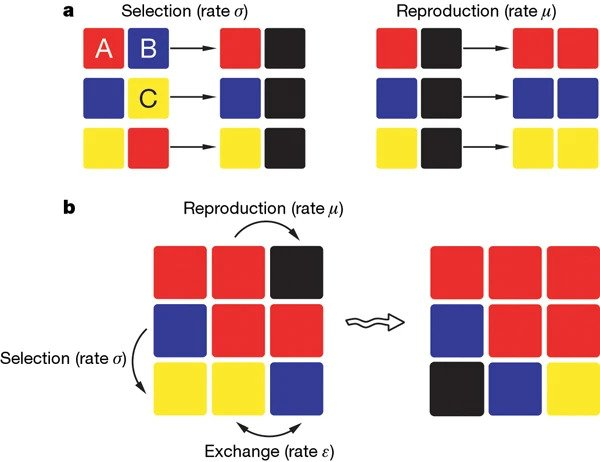
\includegraphics[width=\linewidth]{rules.jpg}
\captionof{figure}{}
\end{minipage}
\begin{minipage}{0.5\textwidth}
The reactions occur as Poisson processes. We will denote selection at rate $\sigma$ and reproduction at rate $\mu$. Selection reflects the cyclic dominance: A can kill B and this will yield an empty site (black). This is the same as B invades C and C outcompetes A. Reproduction is only allowed on empty neighbouring sites. The exchange reaction is to mimic the movement of the microbes, any individual can either swap position with a neighbouring individual or hop onto an empty neighbouring site. This occurs as a Poisson process of rate $\epsilon$.
\end{minipage}\\\\
Within this setting, using the theory of random walks\cite{rw}, the typical area explored by one mobile individual per unit time through the exchange reaction is proportional to $M=2\epsilon N^{-1}$. The interplay of exchange with selection and reproduction processes sensitively determines which species exist and if they coexist.\\
We defined the unit time as one generation, i.e. the time taken when every individual has reacted on average once. At each simulation step, a random individual is chosen to interact with one of its four nearest neighbours: which one is also randomly determined. To determine which reaction occurs and the corresponding waiting time, i.e. how many exchanges occur between two selections/reproductions, we use an algorithm from Gillespie\cite{alg} and the reaction rates.\\
We set the total waiting time to $t=0.1N^2$. This is because the waiting time $t$ is dependent on the system size $N^2$, and the extinction probability $P_{ext}$ is proportional to the total waiting time until extinction. So to compare between different parameters, we only need to make sure $u=\frac{t}{N^2}$ is the same between all tests\cite{time}.\\
Finally, without loss of generality, to only consider the effect motility has on the system, we fix $\mu=\sigma=1$.

\subsection{one-public-good system}
In a one-public-good system, we introduce two types of microbes instead of the three species in the rock-paper-scissors game in 2.1. The microbes are cooperators and defectors. The cooperators will produce secretions that is beneficial to the neighbouring cells but the action of producing the secretion is not necessarily beneficial to the producer itself as there is a corresponding cost to the action. On the other hand, the defectors do not produce any secretions, they will live off the secretions produced by the cooperators. Both types of microbes are allowed to select, reproduce and exchange.\\
To represent the effect from this, we introduced a fitness function into the model. The fitness $f$ of the microbe affects whether selection or reproduction can occur. In our code, for a reproduction to happen, we require $f > U(0,1)$, where $U(0,1)$ is the uniform distribution; and similarly, for a selection to happen, we require $f_1 > f_2$, where $f_1$ is the fitness of the microbe selected and $f_2$ is the fitness of its randomly chosen neighbour.\\
To calculate the fitness $f$ of a microbe, we use the following formula:
\[\text{fitness} = \text{base rate} - \text{cost} + \text{number of neighbouring cooperators} \times \text{good produced per cooperator}\]
In the fitness formula above, cost represents the cost of producing the secretion, which is a constant $c$ for cooperators and $0$ for defectors. The number of neighbouring cooperators is defined to be the number of cooperators that's in the $3\times 3$ centred at the focal cell.\\
 Another parameter was also introduced and it is the initial density of the lattice, this is defined using the concept of sparsity $s$. $s$ is defined such that:
\[\mathds{P}(L_{(i,j)}\in\{0,1\}) = \frac{2}{s}\]
where $L_{(i,j)}$ is the $(i,j)^{th}$ cell of the lattice and 0,1 represents assignment as a cooperator and defector respectively.\\
We again examine the extinction probability of the defectors and cooperators after $t=0.1N^2$ and observe the density of the two species in the lattice after waiting time of extinction. We have varied the density, fitness to determine their effects on extinction probability vs. motility. From this point onwards, the lattice has also been fixed at $N=100$ to simplify the computing power required to run sufficient simulations. The range of motility used is adjusted accordingly.
\subsection{Chemotaxis and Motility Ratio}
Building on the model from 2.2, the chemotaxis algorithm was developed to mimic the bias the microbes have when moving. The microbes can either move away (chemoaversion) or move towards (chemotaxis) areas with higher concentration of secretions or in our model, cells that have higher fitness.\\
The formula for chemotaxis is:\[\mathds{P}(\text{$L_{(i,j)}$ exchange with $L_{(i+k,j+l)}$})=\frac{f_{(i+k,j+l)}}{\sum_{(k,l)=[(0,1),(0,-1),(1,0),(1,-1)]} f_{(i+k,j+l)}}\]
where $i, j$ are fixed focal cells chosen before the exchange, and $k,l$ the possible neighbouring cells it can exchange with. This formula is used to reflect that on expectation, the microbe on cell $(i,j)$ will move towards the cells with higher concentrations of secretions but it is probabilistically possible for it to still move in other directions.\\
For chemoaversion, we define $f^a_{(i+k,j+l)}$ as the relative aversion fitness of the cell $(i,j)$, it is calculated as \[f^a_{(i+k,j+l)}=1-\frac{f_{(i+k,j+l)}}{\sum_{(k,l)=[(0,1),(0,-1),(1,0),(1,-1)]} f_{(i+k,j+l)}} \]
and therefore
\[\mathds{P}(\text{$L_{(i,j)}$ exchange with $L_{(i+k,j+l)}$})=\frac{f^a_{(i+k,j+l)}}{\sum_{(k,l)=[(0,1),(0,-1),(1,0),(1,-1)]} f^a_{(i+k,j+l)}}\]
Simulations were also done with motility ratio, this is when the cooperators and defectors have different exchange rate $\epsilon$.\\

\subsection{two-public-good system}
After having tested with one-public-good system, we continued the work on the main focus, a two-public-good system. Whilst the parameters and method of collecting the data has maintained mostly the same, two new species were introduced, the cross-feeders, which are represented as $(1,0)$ and $(0,1)$, this shows which good they secrete. Cooperators and defectors are therefore now represented as $(1,1)$ and $(0,0)$.\\
A death rate has also been introduced to simulate the dying process of the cells, which can occur when the fitness of the cell is sufficiently low. The fitness function is adapted so we take influence of the good produced as the minimum of them in the neighbourhood of the focal cell.\\
Whilst the mathematical nature of the model have not changed, the introduction of a second type of good required a substantial amount of coding to adapt the program correctly to deal with the extra species and type of goods as well as a substantial amount of time to determine the constants required as there is now an increased number of parameters one needs to fix when experimenting.\\
This extended the amount of computational power required for simulation, and hence it is important to utilise computers with a large number of cores and multiprocessing to increase the number of simultaneous simulations one can run.\\
Initial experiments were run to determine the effect of motility on extinction probability at different conditions (base fitness, cost of production, initial density of lattice, death rate).\\
Density-dependent motility has also been introduced, where the exchange rate $\epsilon$ between the microbes would decrease significantly when the lattice density of cells is high in the local neighbouring region of the focal cell or globally. The local areas tested were $ 3-7 \times 3-7$. The critical density we looked at were between $50\%-90\%$.These simulations were first carried out on simpler one-public-good system.

\section{Results}
\subsection{Reproducibility}
After developing the initial base model, simulations were run to compare the results with \cite{rps}. The original work computed $P_{ext}$ as a function of the mobility M (and $\sigma$ = $\mu$ = 1), and show results for different system sizes with lattice length N: N = 20 (green), N = 30 (red), N = 40 (purple), N = 100 (blue), and N = 200 (black) over 50-200 simulations.\\
We computed 50 simulations per data point with N = 20 (blue), N = 30 (orange), N = 40 (green) and N = 100 (red). All cells of the lattice is filled randomly at $t=0$.\\
\begin{figure}[H]
            \centering
            \textbf{Experimental}\par
            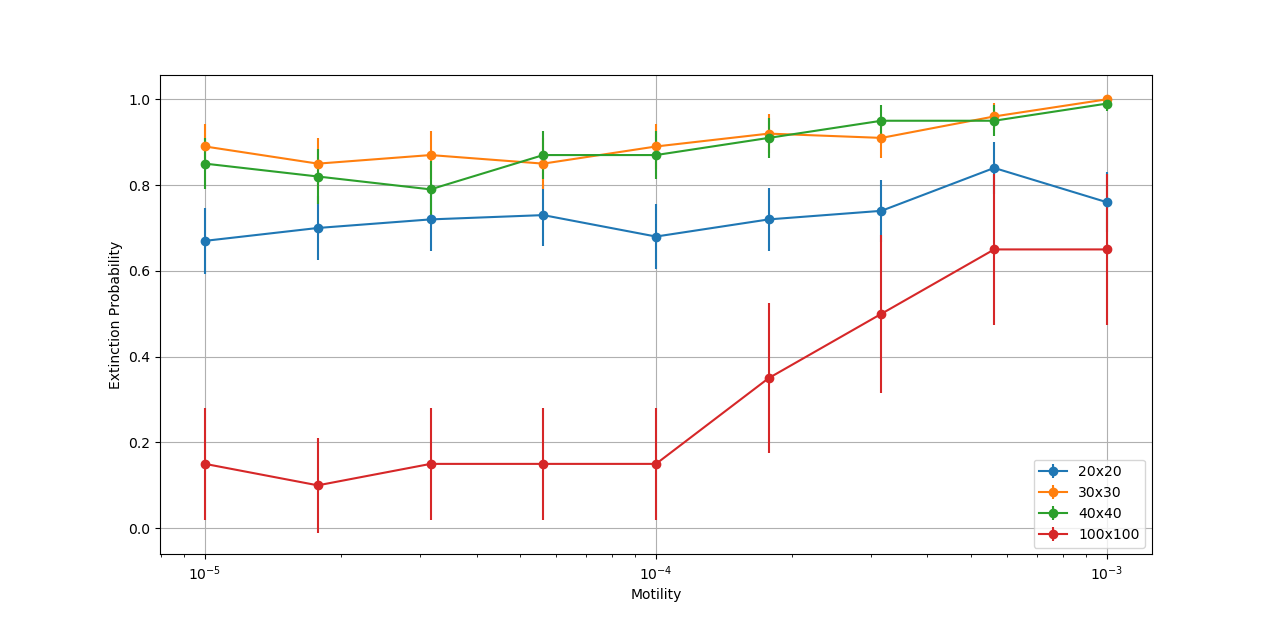
\includegraphics[width=0.75\textwidth]{reproduce.png}
            \caption{Simulation using base model}
\end{figure}
\begin{figure}[H]
            \centering
            \textbf{Comparison}\par
            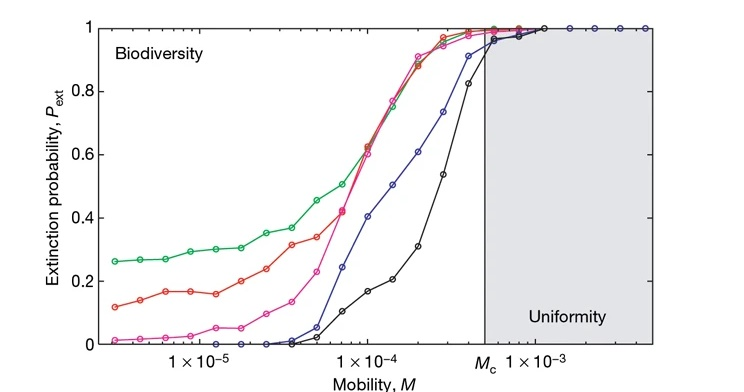
\includegraphics[width=0.75\textwidth]{comparison.jpg}
            \caption{Original graph from \cite{rps}}
\end{figure}
\noindent The broad pattern observed matches the results from the comparison, which is the extinction probability increases the quickest transitioning from $M=10^{-4}$ to $M=10^{-3}$. In the experiments we ran though, whilst the N = 100 curve fits well with original equivalent, we saw that the extinction probability for N = 20 to N = 40 haven't changed significantly with the change of M, and in fact the extinction probability has increased from N = 20 to N = 40, which is the opposite of what occurred in the original work.\\
This is because the density of the three species oscillates as $t$ increases, and the magnitude of the peak of the density curve also increased, so at small N. This means when the magnitude is too large, the trough would have been lower than 0, which is not physically possible and thus extinct prematurely. Thus, the base system is much susceptible to change in size of lattice instead of the motility the cells are moving at.\\
Experiments at larger lattice size (N = 200, plotted separately) and animations confirmed that at larger scale the results are very similar to the original work and similar spatial patterns were observed. To see the animations, go to GitHub repository and animation folder.

\subsection{one-public-good system}
Therefore, to make sure the model is valid and reduce computation hours, we fixed N = 100 from here onward and converted M to the correct exchange rate $\epsilon$ using the equation in section 2.1. N = 100 is chosen because it best reflects the spatial structure of the system 
and is easier to compute since the algorithm is $\mathcal{O}(N^4)$. Any increase in the system size will disproportionally increase the time needed.\\
We selected the amount of good produced per cooperator to be $0.1$, and with further experiments, decided to use three levels of base rate, cost of production and sparsity to reflect the different effect they have on the motility vs. extinction probability graph. The three levels will be high, medium and low, and they are defined as following:
\begin{itemize}
    \item base rate
    \begin{itemize}
        \item low: 0.05
        \item medium: 0.1
        \item high: 0.2
    \end{itemize}
    \item cost of production
    \begin{itemize}
        \item low: 0.005 (5\%)
        \item medium: 0.01 (10\%)
        \item high: 0.05 (20\%)
    \end{itemize}
    \item sparsity
    \begin{itemize}
        \item low: 10
        \item medium: 50
        \item high: 100
    \end{itemize}
\end{itemize}

\noindent Figure 4 below is used as the control graph to compare the effects from the three parameters. It is made using 25 samples per data point where the data points' exchange rate are logarithmically chosen from $10^{-3}$ to $10$, there are 9 data points in total. The cooperator's curve is in orange and defector's curve is in blue.\\
We observe that at low motility, cooperators perform well and defectors almost always reach extinction. This is because we have a low initial density (high sparsity), so there are sufficient space and time for the cooperators to reproduce and form large clusters to repel the defectors. When this can be achieved, the cooperators will 'win'. \\
However, as the exchange rate increases, the time for cooperators to reproduce and form a sufficiently large cluster is shortened, as now the defectors can move faster and hence can easily find cooperators which secretions they can use for reproduction without having the produce them. In these cases, the defectors will 'win'. The critical region is between $0.1$ and $1$, which is when the extinction probability changes at the highest rate and this corresponds to the critical region in figure 3 when the exchange rate is converted.
\begin{figure}[H]
    \centering
    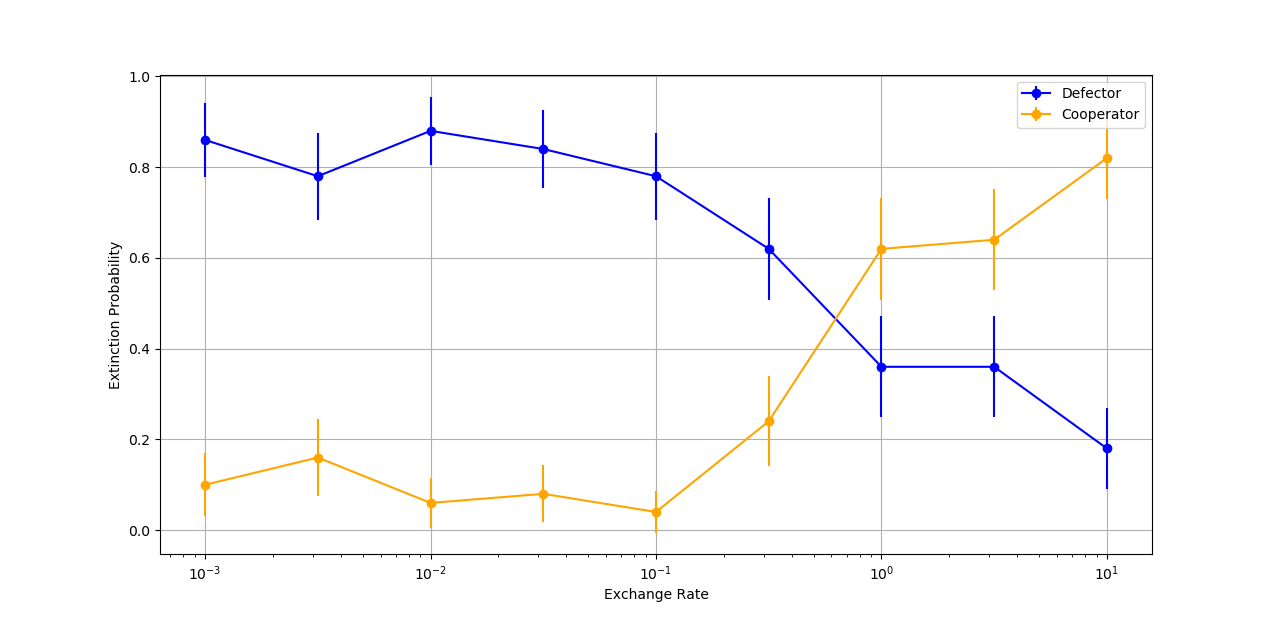
\includegraphics[width=0.8\textwidth]{Repeated Graph.png}
    \caption{Motility vs. Extinction Probability, high base rate, high cost, high sparsity}
\end{figure}
\noindent We proceed to sketch 9 graphs, each with fixed base rate and sparsity, and 6 curves each graph, representing the extinction probability of defectors and cooperators at the 3 levels of cost of production.\\
\begin{figure}[H]
            \centering
            \textbf{High sparsity, high base rate}\par
            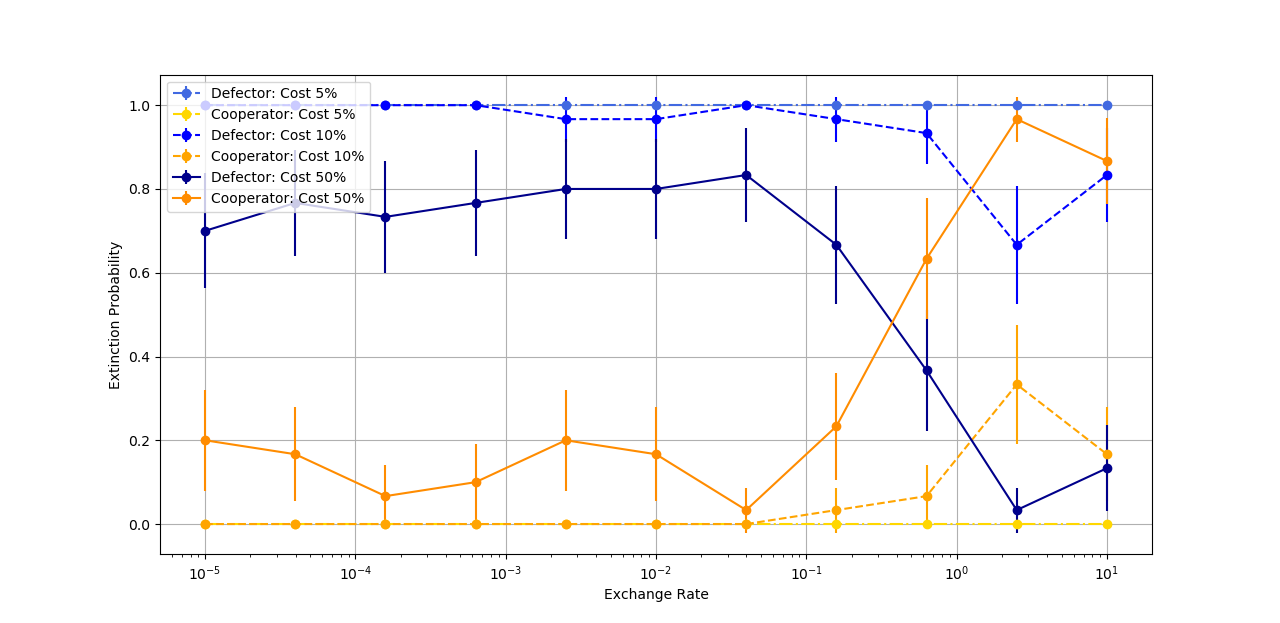
\includegraphics[width=0.73\textwidth]{Low Density, High Basal Fitness.png}
            \caption{}
\end{figure}
\begin{figure}[H]
            \centering
            \textbf{High sparsity, medium base rate}\par
            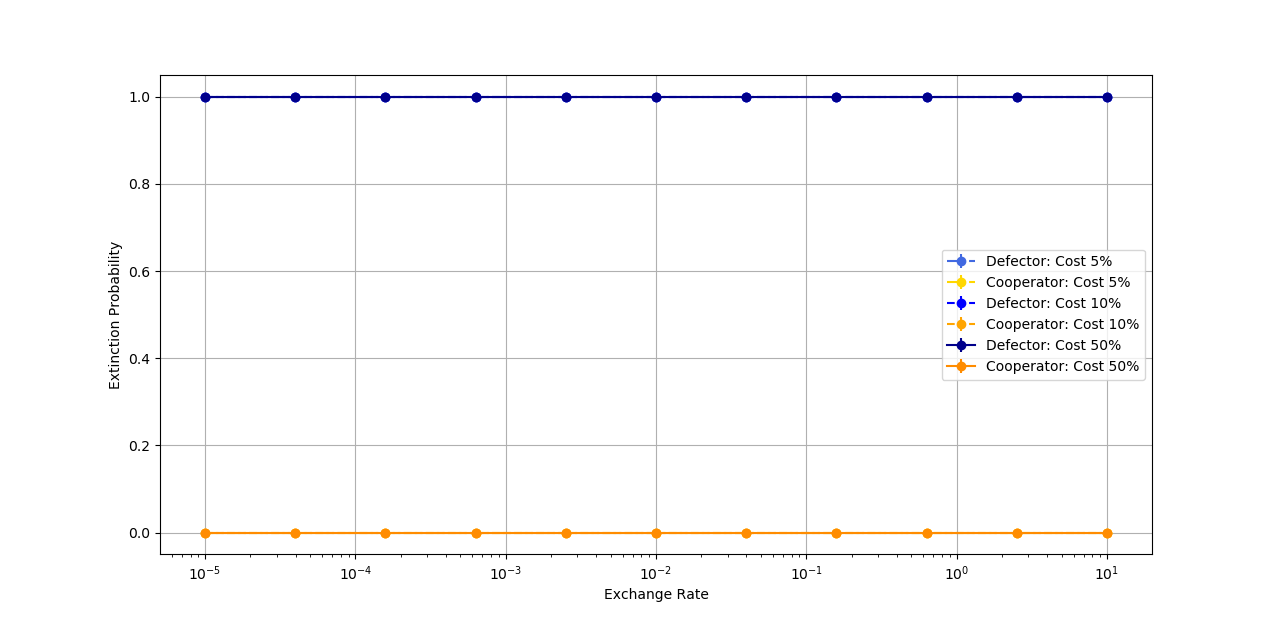
\includegraphics[width=0.73\textwidth]{Medium Density, Low Basal Fitness.png}
            \caption{}
\end{figure}
\begin{figure}[H]
            \centering
            \textbf{High sparsity, low base rate}\par
            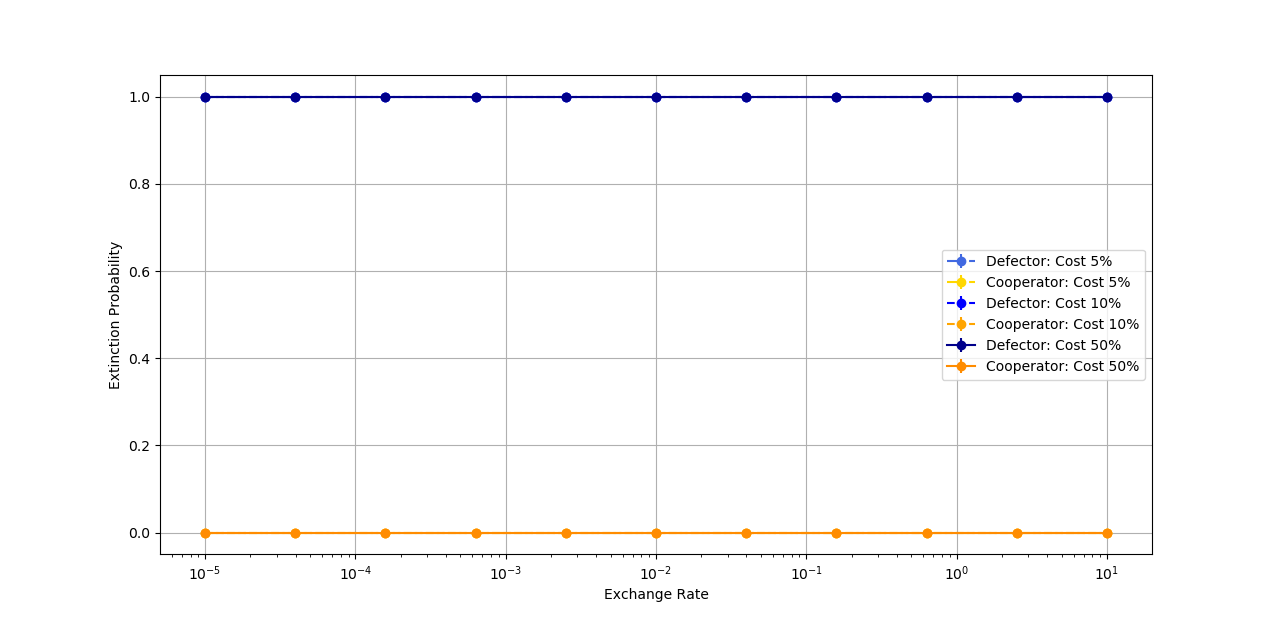
\includegraphics[width=0.73\textwidth]{Medium Density, Low Basal Fitness.png}
            \caption{}        
\end{figure}
\begin{figure}[H]
            \centering
            \textbf{Medium sparsity, high base rate}\par
            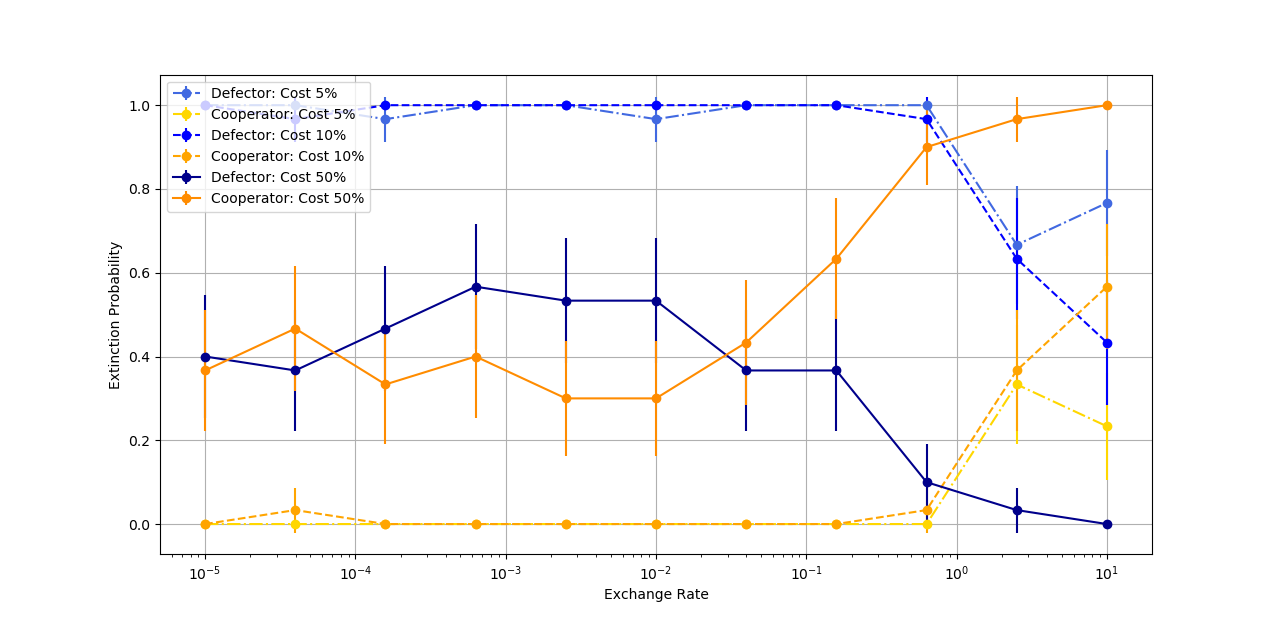
\includegraphics[width=0.73\textwidth]{Medium Density, High Basal Fitness.png}
            \caption{}
\end{figure}
\begin{figure}[H]
            \centering
            \textbf{Medium sparsity, medium base rate}\par
            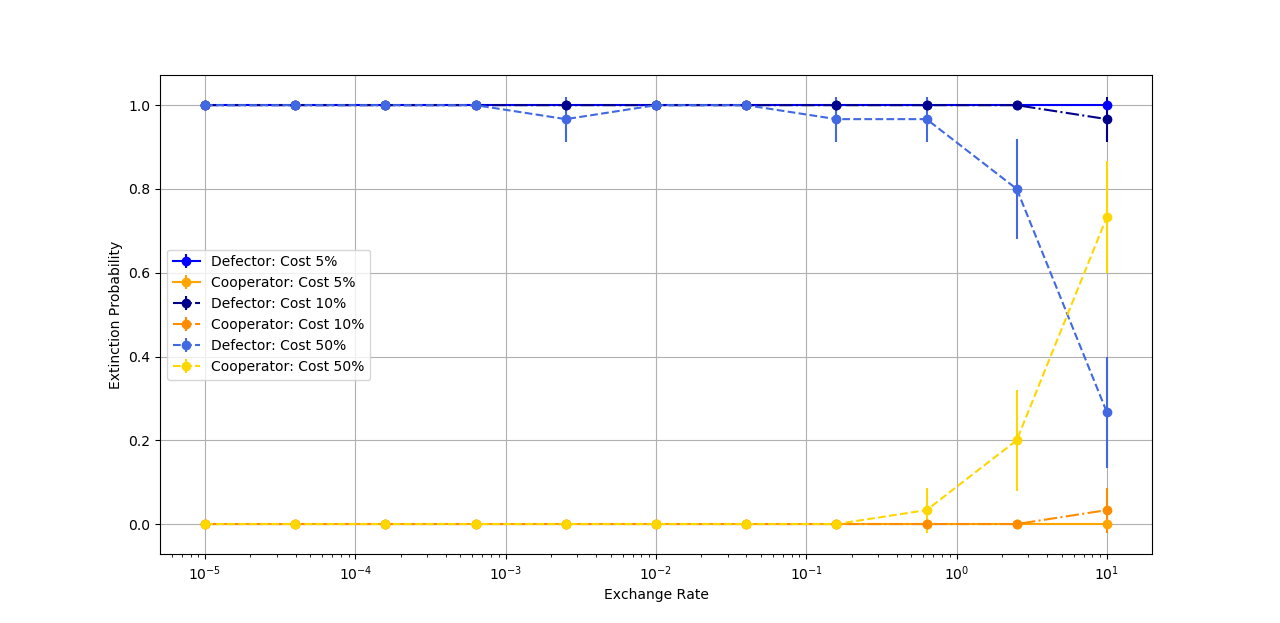
\includegraphics[width=0.73\textwidth]{Medium Density, Medium Basal Fitness.png}
            \caption{}
\end{figure}
\begin{figure}[H]
            \centering
            \textbf{Medium sparsity, low base rate}\par
            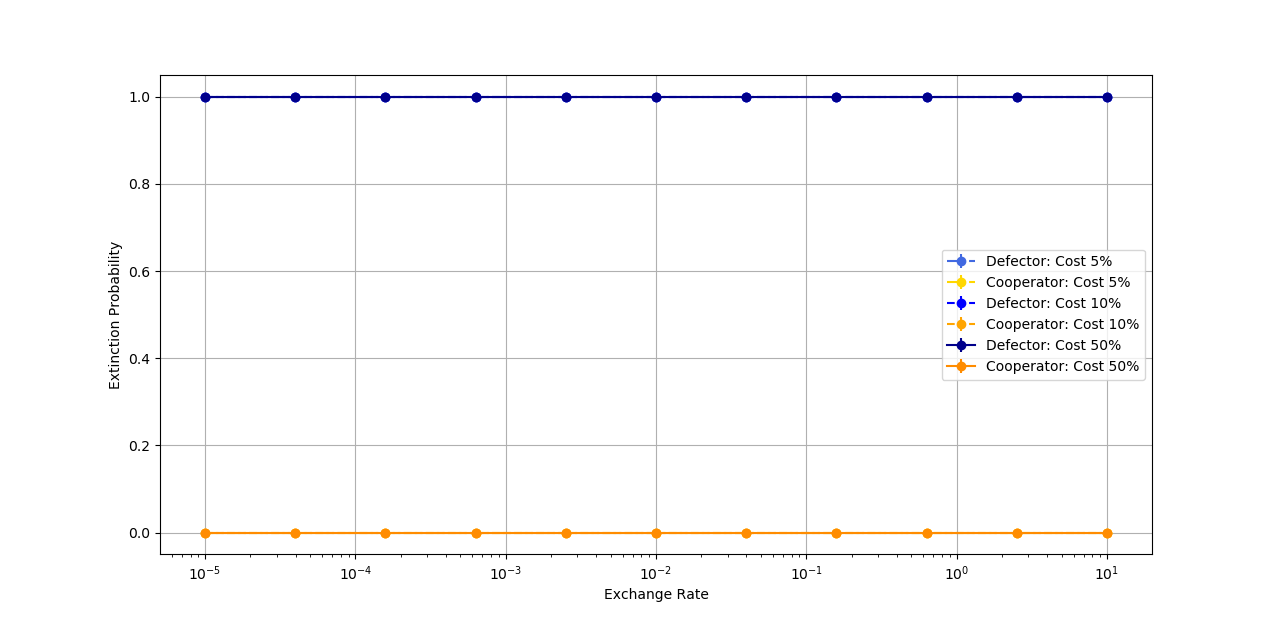
\includegraphics[width=0.73\textwidth]{Medium Density, Low Basal Fitness.png}
            \caption{}        
\end{figure}
\begin{figure}[H]
            \centering
            \textbf{Low sparsity, high base rate}\par
            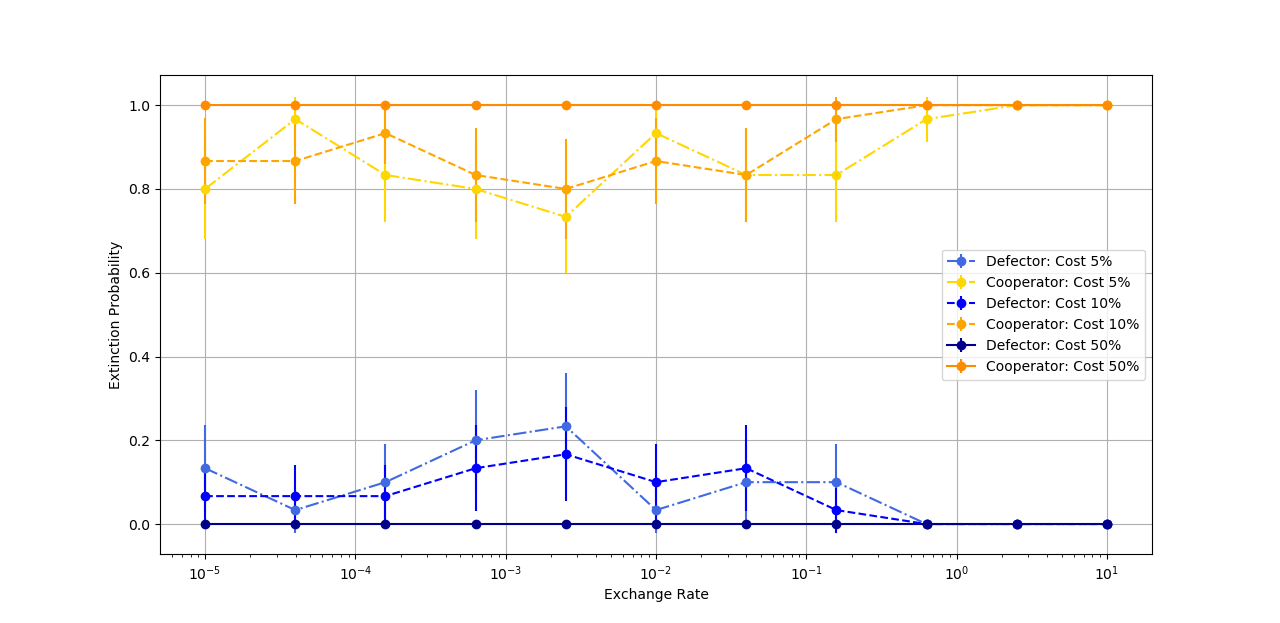
\includegraphics[width=0.73\textwidth]{High Density, High Basal Fitness.png}
            \caption{}
\end{figure}
\begin{figure}[H]
            \centering
            \textbf{Low sparsity, medium base rate}\par
            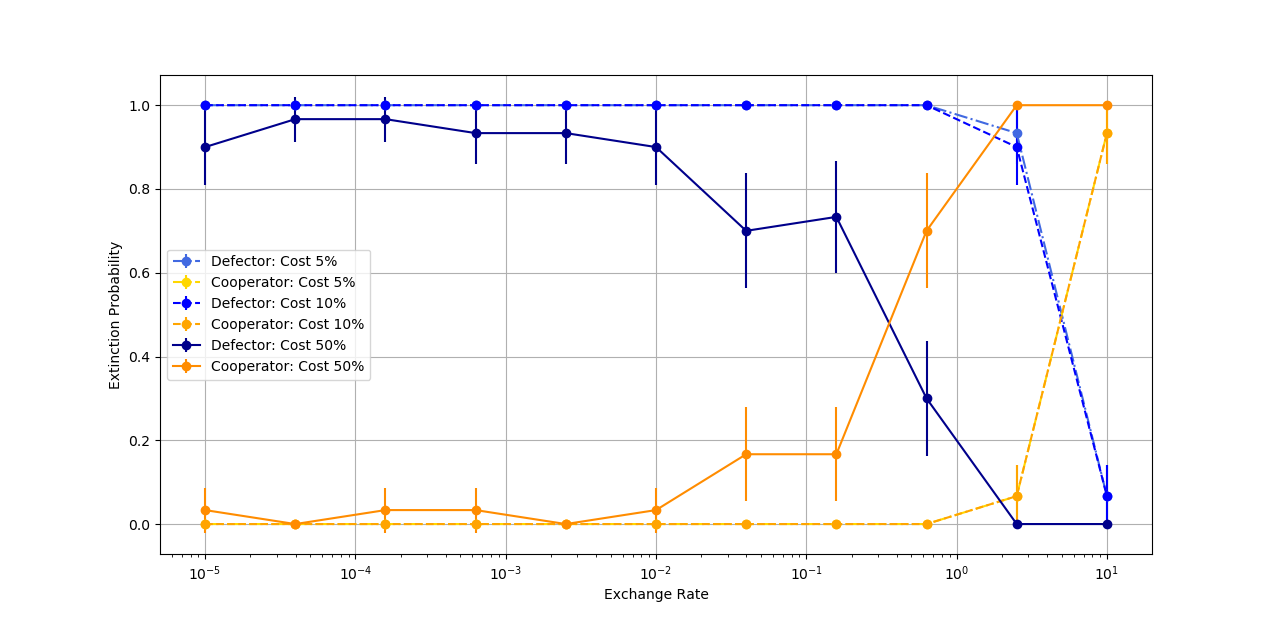
\includegraphics[width=0.73\textwidth]{High Density, Low Basal Fitness.png}
            \caption{}
\end{figure}
\begin{figure}[H]
            \centering
            \textbf{Low sparsity, low base rate}\par
            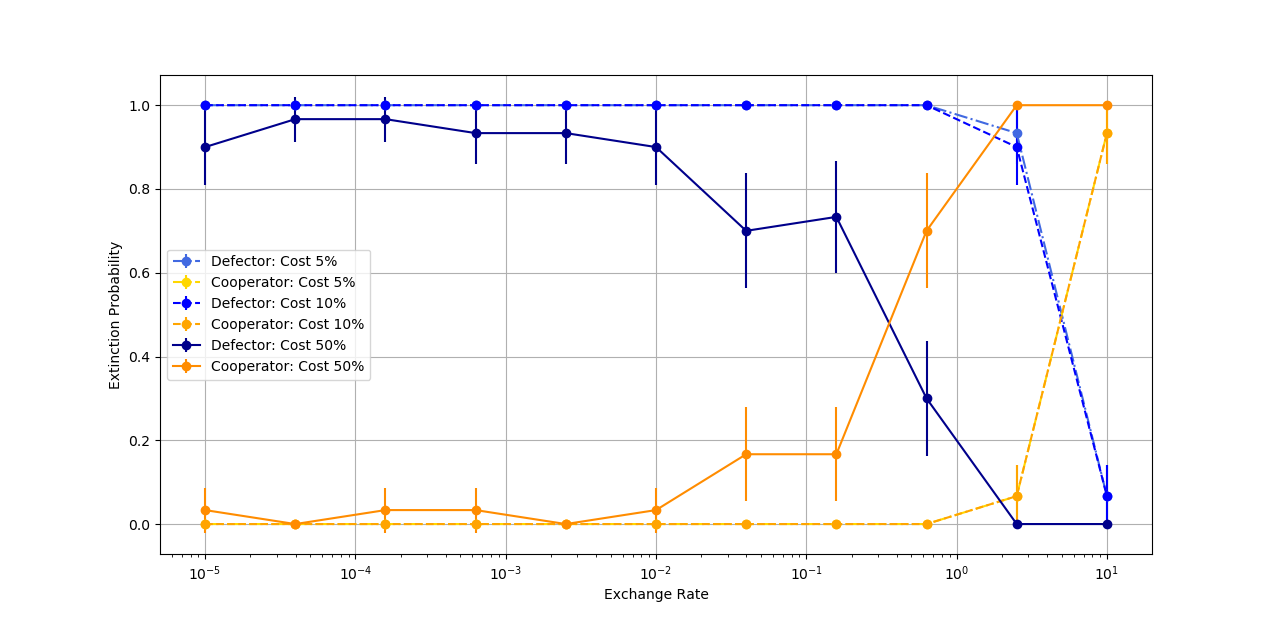
\includegraphics[width=0.73\textwidth]{High Density, Low Basal Fitness.png}
            \caption{}        
\end{figure}

\noindent We first observe from figure 5,8,9,11,12,13 that when the sparsity and base rate is fixed. Increasing the cost of production benefits the defectors and disadvantages the cooperators. This is simply because a higher cost means the cooperators need to be in larger clusters of itself to perform well, otherwise the defector will have a higher fitness than the cooperator since they have no cost and can use the public good for free.\\
This effect is maximised at low sparsity (high initial density), since the cooperators have less time to find others and reproduce and the defectors can easily benefit from the abundance of cooperators around them.\\
We also note from figure 5,8,11 that decreasing the sparsity benefits the defectors. We note when sparsity is reduced from high to medium, the 'Defectors: Cost 50\%' line translated down by roughly 0.2 at all data points especially at slower exchange rates. And in figure 11, the defectors 'wins' at all exchange rates simulated even though in other figures, the cooperators have a lower extinction probability at slow exchange rates.\\
This is because decreasing the sparsity increases the probability the microbes meeting other cells when $t$ is small, and this reduces the effect from the reproduction by themselves (where cooperators have fitness 0.25 and defectors 0.2) and increases the effect from reproduction/selection with others (if cooperator with defector, then cooperator has fitness 0.25 and defector 0.3), so the defector would 'kill' cooperator and reproduce faster when it meets a cooperator.\\
Furthermore, we note from figure 8,9,10 that a low base rate benefits the cooperators. This is because a lower base rate increases the relative value of the good produced in the fitness equation. More importantly, this means the defectors cannot reproduce at a high rate when it's not surrounded by a good number of cooperators. For example, at high sparsity and high cost, the defector only has a fitness of 0.05 when it's by itself whereas the cooperator has a fitness of 0.1, so double the reproduction rate than defectors.\\
So to conclude, cooperators like high sparsity, low base rate and low cost; and defectors like low sparsity, high base rate and high cost.

\subsection{Chemotaxis and Motility Ratio}
Building on results in 3.2, most of our further results chose the parameters to be high sparsity and high base rate. This is so we can observe the difference the new algorithm have on the system.\\
Chemotaxis and chemoaversion and motility ratio are introduced separately. For the former two, simulations were only ran for the stated conditions and for the three levels of cost. Each point on the graphs contains 15 samples. This is a very small number of data points and more simulations need to be ran.\\
When chemotaxis algorithm was implemented, we observe that the defectors seem to have performed better than in figure 5. With the extinction probability of defectors being 0.4 when the exchange rate is $10^{-2}$ and the intersects the extinction probability curve of cooperators. This occurred at a much lower exchange rate than in figure 5, which was between $\epsilon=0.1$ to $\epsilon=1$. Since there are no further data, it's hard to predict what would've happened to the system at faster exchange rate, but from other graphs previously sketched, we suspect that it will demonstrate a similar pattern to figure 5 but both curves slightly shifted left.\\
The reason for the lower extinction probability for defectors is that chemotaxis benefits defectors and enables them to move towards areas with high concentration of cooperators easily. This therefore decreases the difficulty of defectors to reproduce by increasing its fitness.\\
Therefore, we predict the exact opposite would happen when chemoaversion is implemented and this is shown in figure 15.\\
\begin{figure}[H]
    \centering
    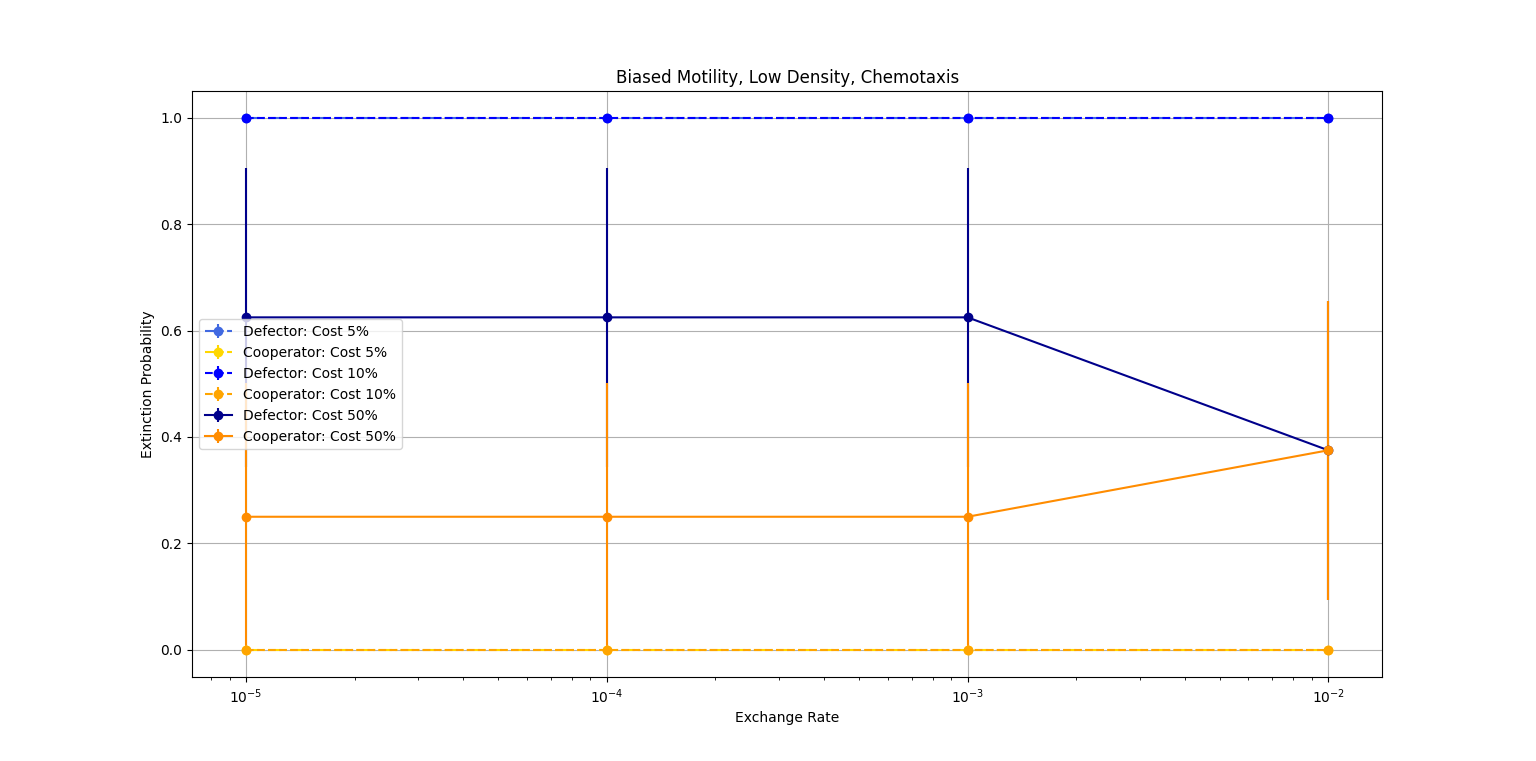
\includegraphics[width=0.65\textwidth]{Biased Motility Low Density Chemotaxis.png}
    \caption{Motility vs. Extinction Probability with chemotaxis, different cost at high sparsity, high base rate}
\end{figure}
\begin{figure}[H]
    \centering
    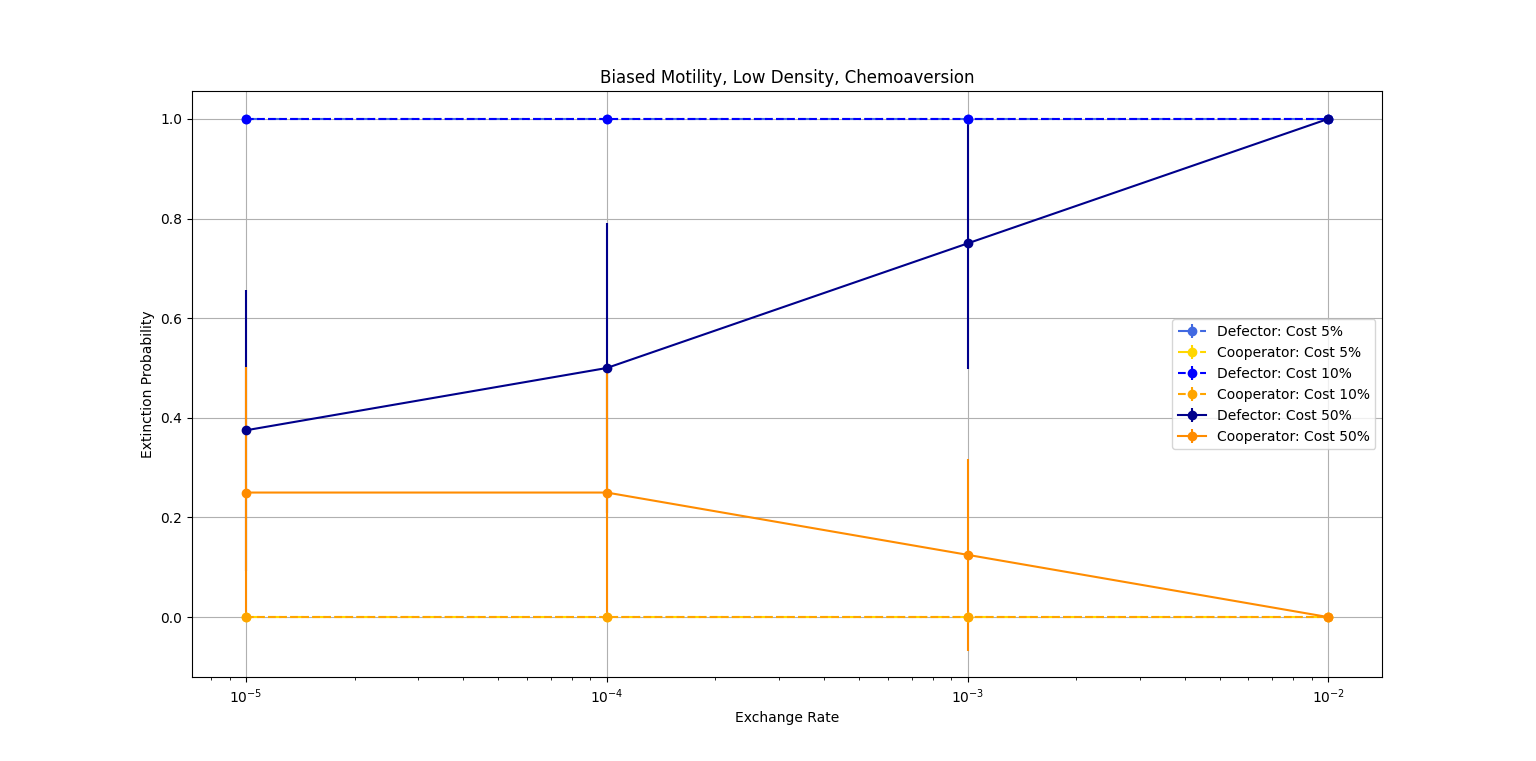
\includegraphics[width=0.65\textwidth]{Biased Motility Low Density Chemoaversion.png}
    \caption{Motility vs. Extinction Probability with chemoaversion, different cost at high sparsity, high base rate}
\end{figure}
\noindent For chemoaversion, we observe that as exchange rate increases, the extinction probability of defectors actually increase, and decrease for cooperators. This is because at slower exchange rate, the effect of motility is negligible and the evolution of the system is mostly dependent on selection and reproduction alone but as the rate increases, it plays more of an important role, and now defectors are actively moving away from resources they need and this lowered their mean fitness.\\
\begin{figure}[H]
    \centering
    \textbf{Low sparsity}\par
    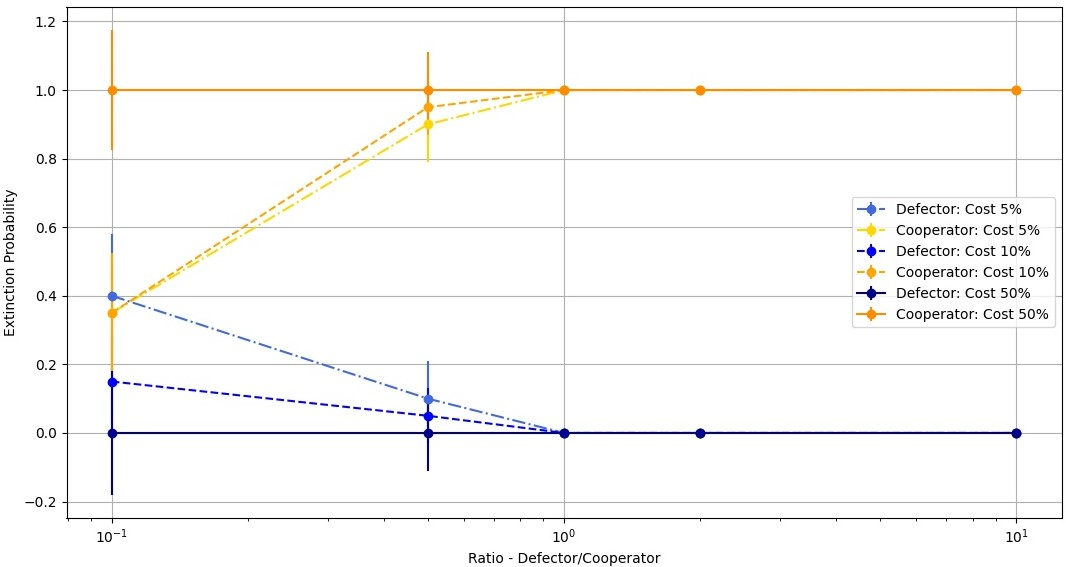
\includegraphics[width=0.55\textwidth]{Motility_Ratio_High_Density.jpg}
    \caption{Motility vs. Extinction Probability with motility ratio, different cost at low sparsity, high base rate}
\end{figure}
\begin{figure}[H]
    \centering
    \textbf{High sparsity}\par
    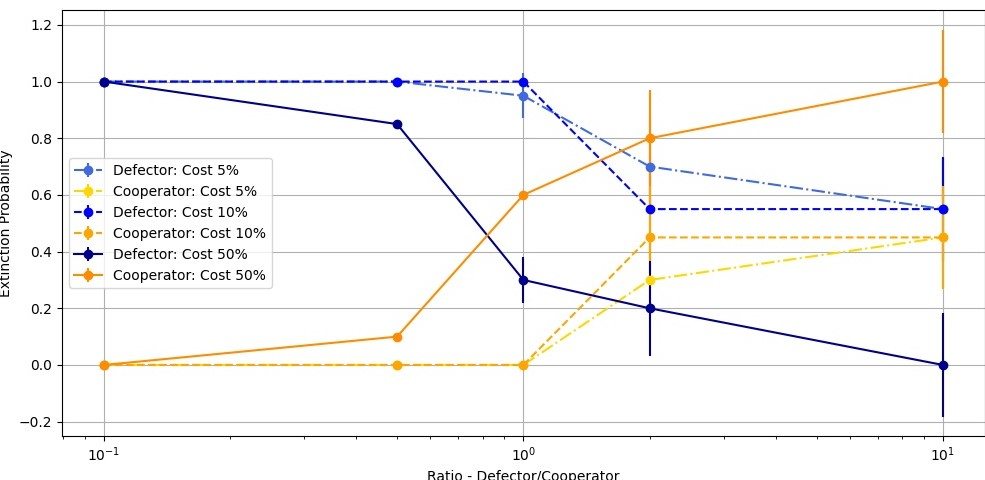
\includegraphics[width=0.65\textwidth]{Motility_Ratio_Low_Density.jpg}
    \caption{Motility vs. Extinction Probability with motility ratio, different cost at high sparsity, high base rate}
\end{figure}
\noindent For the latter (motility ratio), we carried out simulations on high and low sparsity and high base rates with different costs.\\
Each data point had 30 samples. The ratios tested was $r\in[0.1,0.5,1,2,10]$, i.e. defectors moves $r$ times faster than cooperators. The base cooperator exchange rate is set to be $\epsilon=1$.\\
We note at both sparsity, defectors' extinction probability decreases as exchange increases, this is as expected, since high exchange rate benefits defectors and defectors are moving faster than cooperators at ratios larger than 1 and vice versa. The difference between motility ratio and just changing the exchange rate of both species is that when we introduce the motility ratio, the rate of change between each data point is increased, i.e. there is a more significant effect to the extinction probability of the species. This is because the difference in moving speed gives a huge advantage to defectors as they can now 'hunt' any clusters of small cooperators and take away the space they need to survive at early stages of the evolution.\\
When we ignore the effect of motility ratio and look at just the data point at ratio 1 in figure 17, i.e. when both defectors and cooperators move at exchange rate 1, the data is the same as in figure 5.\\

\subsection{two-public-good system}
Some results were done on partial systems with cross-feeders and cooperators or cross-feeders and defectors. They are not shown here as most are repetitive work of section 3.2 and 3.3.\\
Some simulations were also run on the effect of death rate, this is not shown but results can be found in GitHub and shared folders. The death rate is set to be 0.04 in following results.\\
A significant amount of individual tests were carried out to determine the values at which cross-feeders can outperform cooperators and defectors. Readers are recommended to use small scale individual simulation tests to locate the range of possible range of conditions, due to time constraint, only one set of conditions were tested thoroughly in this project.\\
In figure 18, the orange and yellow curves represent the cross-feeders (1,0) and (0,1) respectively. The blue curve represents the cooperators and red curve represents the defectors. The parameters chosen were:
\begin{itemize}
    \item Good per cooperator: 0.1
    \item cost of production per cooperator: 0.1
    \item Good per cross-feeder: 0.3
    \item Cost of production per cross-feeder: 0.01
    \item sparsity: 50
    \item base rate: 0.05
    \item death rate: 0.04
\end{itemize}
\begin{figure}[H]
    \centering
    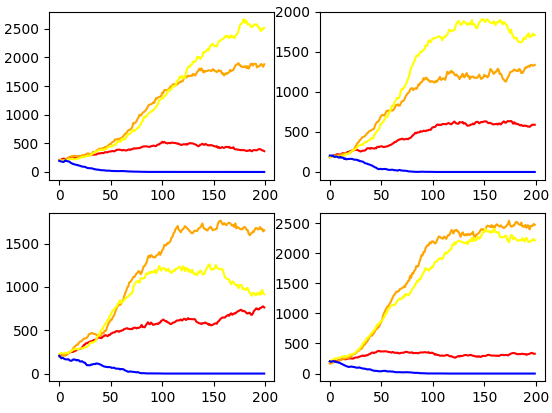
\includegraphics[width=0.5\textwidth]{G1 0.3 G0 0.1 C1 0.01 C0 0.1 sparsity 50 ex 0.1.png}
    \caption{time step vs. density of species in chosen individual simulations at exchange rate 0.1}
\end{figure}
\noindent We see from the individual simulations at exchange rate 0.1 that cross-feeders actually out-perform both cooperators and defectors. This led us to sketch motility vs. extinction probability graphs with sparsity = 50, 75, 100 respectively.
\begin{figure}[H]
    \begin{minipage}[b]{0.5\linewidth}
      \centering
    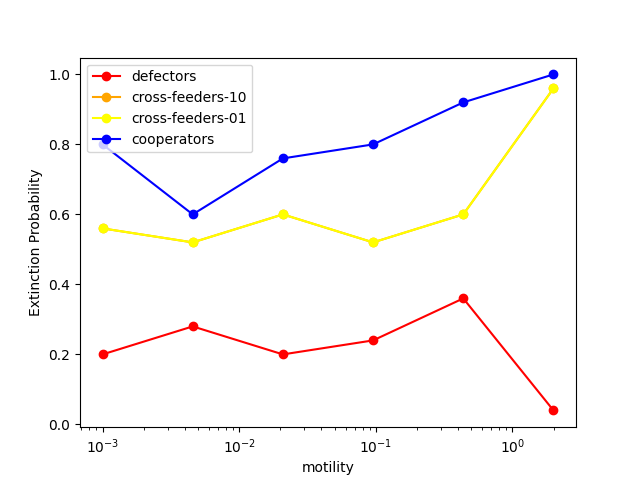
\includegraphics[width=\textwidth]{extinction_prob_high_density.png}
    \caption{sparsity = 50}
        \end{minipage}
        \hfill
    \begin{minipage}[b]{0.5\linewidth}
    \centering
    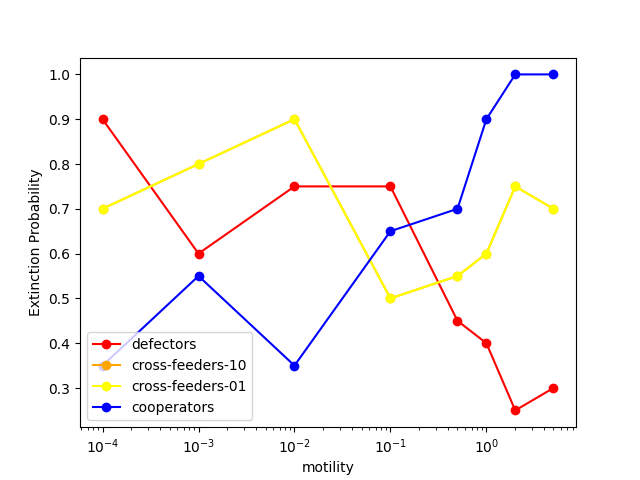
\includegraphics[width=\textwidth]{extinction_prob_medium_density.png}
    \caption{sparsity = 75}
        \end{minipage}
\end{figure}
\noindent This shows us even though in individual tests cross-feeders have performed well at sparsity = 50, 1500 time steps was not sufficient for the defectors to extinct, in fact they consistently perform better than the other three species as low sparsity benefits defectors by reducing distance they need to travel.\\
When sparsity = 75 however, the cross-feeders did perform better around $\epsilon=0.1$, though more samples at more exchange rates needed to be drawn.
\begin{figure}[H]
    \centering
    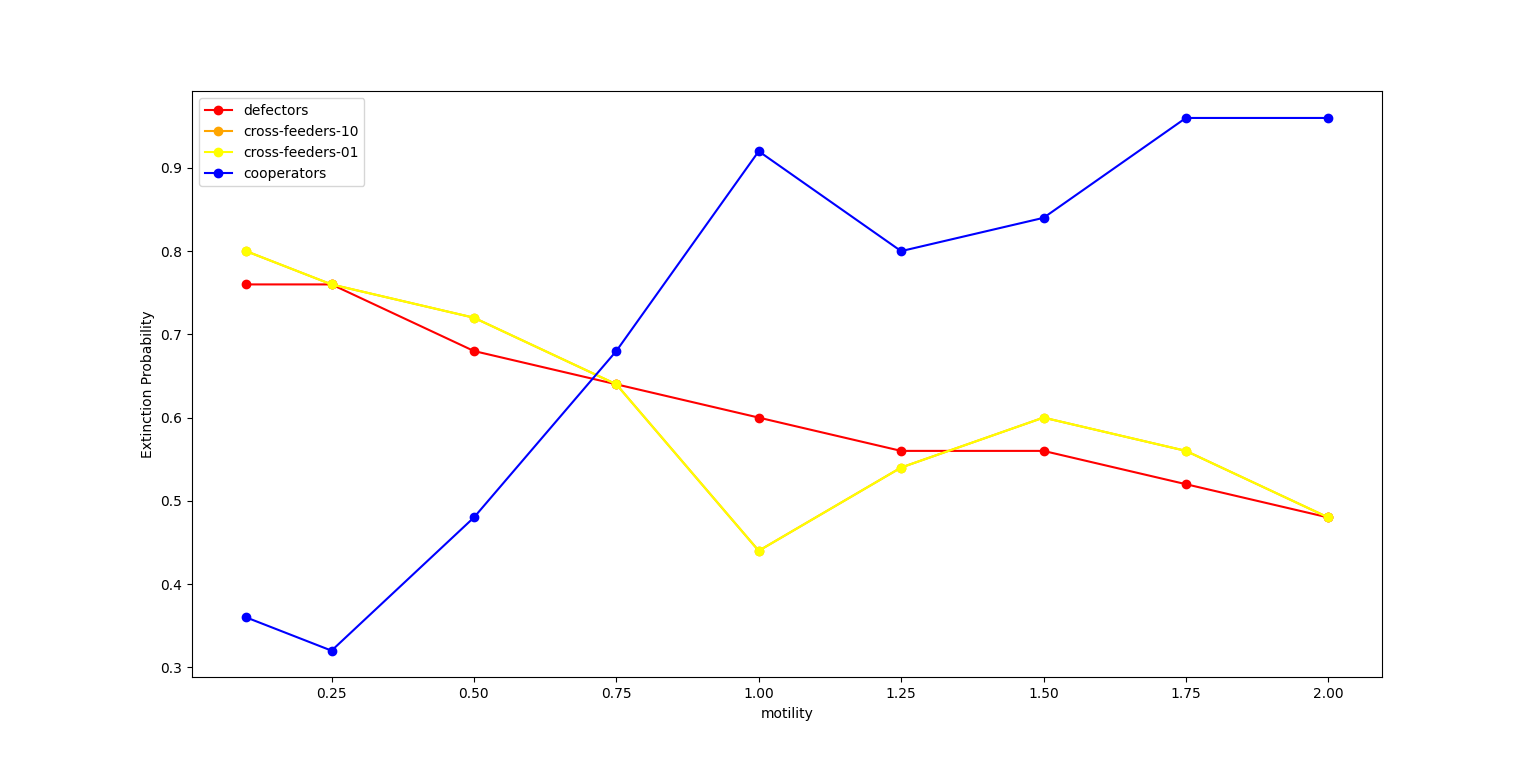
\includegraphics[width=\textwidth]{extinction_prob_low_density.png}
    \caption{sparsity = 100}
\end{figure}
\noindent At sparsity = 100, 40 samples were used for each data point from $\epsilon=0.1$ to $\epsilon=2$. We observe that when the exchange rate is between 0.75 and 1.25, the cross-feeders are performing better than both cooperators and defectors. This is an encouraging sign that cross-feeding can be beneficial in ecoevolutionary systems.\\
Again, more experiments needed to be done, and probably at a slightly lower sparsity as lowering sparsity should translate the defectors curve upwards and give the cross-feeders more advantage.

\subsection{Density-Dependent Motility}
We only had time to experiment with density-dependent motility on one-public-good system, though the results are encouraging and the introduction of such, especially local density-dependent motility would provide further advantage to cross-feeders.\\
For both local and global density constraints, the microbes will move at normal exchange rate initially, but when the local/global density reach a given threshold, the exchange rate is set to $10^{-3}$.
\begin{figure}[H]
    \centering
    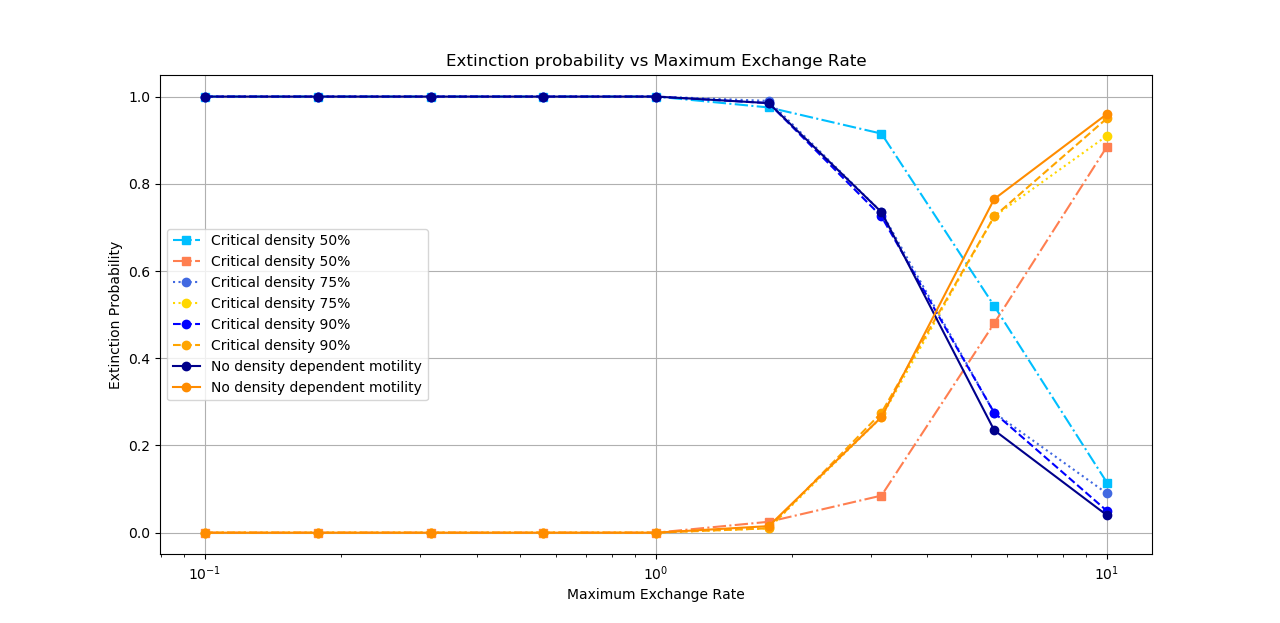
\includegraphics[width=0.7\textwidth]{global density dependence - low initial density, medium basal fitness, high cost.png}
    \caption{global density}
\end{figure}
\noindent In the less important case of global density constraints, we observe that decreasing critical density provides a small advantage for cooperators at the transition exchange rates, i.e. where $\epsilon=1$ to $\epsilon=10$. The advantage is bigger as the critical density is lower from 100\% to 50\%. This is because slower exchange rate benefits cooperators.\\
In the more important case of local density constraints, as it is a better reflection of the in-life situations, we judged the critical density on the neighbouring $7 \times 7$ area around the focal cell. The parameters were:
\begin{itemize}
    \item base rate: 0.15
    \item death rate: 0.05
    \item good per cooperator: 0.1
    \item cost of production: 0.09
    \item sparsity: 100
\end{itemize}
\begin{figure}[H]
    \centering
    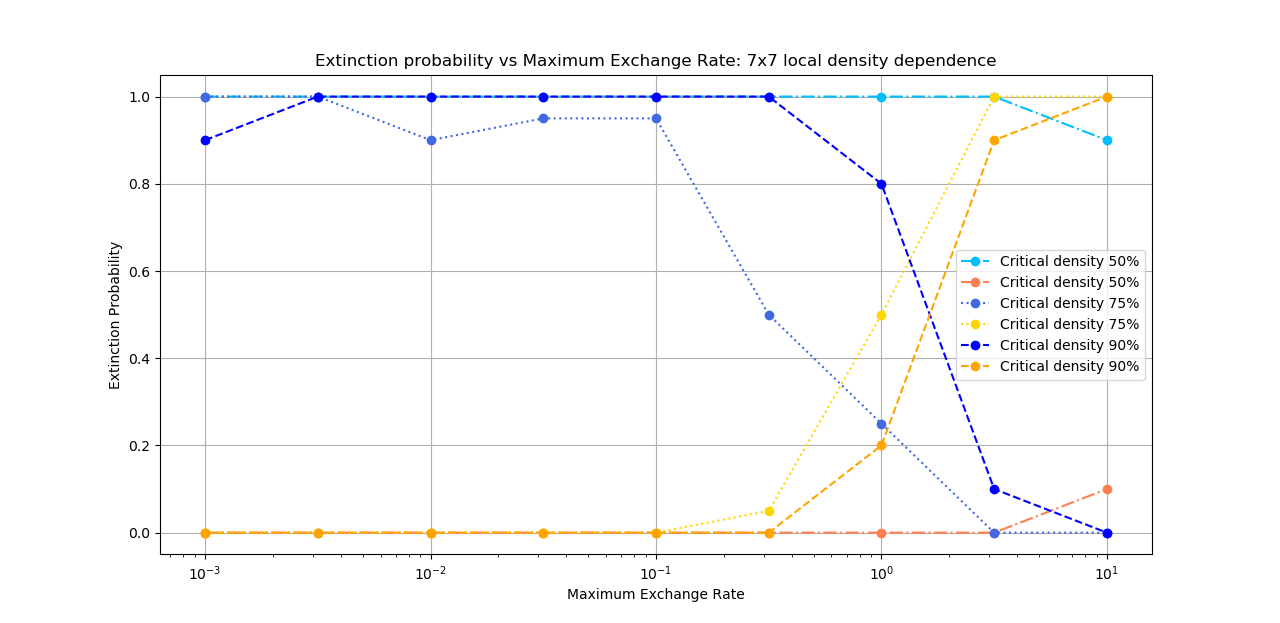
\includegraphics[width=0.9\textwidth]{local 7x7 density dependence - low initial density.png}
    \caption{local density}
\end{figure}
We observe that there is as critical density decreases, the extinction probability in the transition zone (near $\epsilon=1$) for defectors first decreases when critical density is lowered from 90\% to 75\% but then increased when critical density is further lowered to 50\%. This could be due to local clusters having optimal levels of fitness at 75\%, though experiments need to be done to explain this phenomenon and unfortunately, there wasn't enough time to do that.\\\\
\noindent To further illustrate this point, a sketch (figure 24) of defector extinction probability vs. threshold density is plotted at three choices of base rate, at 0.1, 0.15 and 0.2 respectively at exchange rate 1.\\
At base rate = 0.15, which is what figure 23 was based on, we note that there is a sharp decrease at around 63\% where the extinction probability dropped from 1 to 0.15 then slowly increases as the threshold density increases to 100\%. 
\begin{figure}
    \centering
    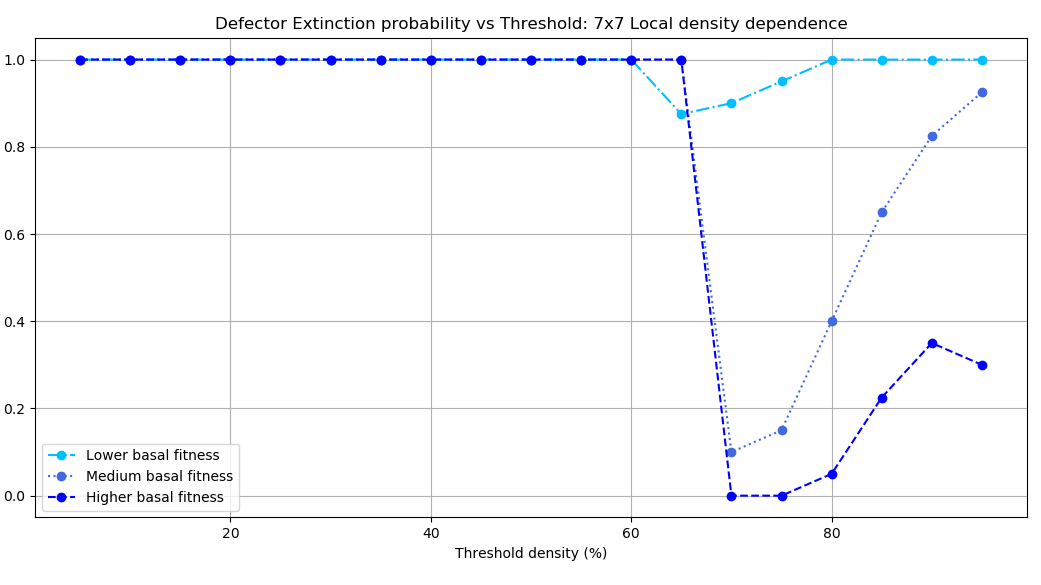
\includegraphics[width=0.8\textwidth]{local 7x7 density dependence - threshold vs defector extinction.png}
    \caption{}
\end{figure}


\section{Conclusion and Discussion}
\subsection{one-public-good system}
From results in section 3.2, 3.3, we have tested on a range of different parameters and their respective effects on the ecoevolutionary system. With the help of figures 5-13, we are able to determine the effect of following:
\begin{itemize}
    \item base rate: Increasing base rate benefits defectors
    \item sparsity: Increasing sparsity benefits cooperators
    \item cost of production: Increasing cost benefits defectors
    \item motility ratio: Large ratio of defector exchange rate to cooperator exchange rate benefits defectors with more significant effect than increasing the exchange rate for both alone
\end{itemize}
We were able to provide some partial evidences to the effect of chemotaxis and chemoaversion and that they advantages and disadvantages defectors respectively.\\
We were not able to collect more data on chemotaxis and chemoaversion mostly due to time constraint since the more algorithm we introduce, the longer their computational time will be. Thus, to be able to have enough time studying the two-public-good system, it was decided that this should be at a later date. It is right to suspect that chemotaxis will prove to be important when implemented on the two-public-good system and may provide an advantage for cross-feeders/defectors when adjusted properly.

\subsection{two-public-good system with normal motility}
From results in the section 3.4, we can conclude that at suitable parameters, it is possible for the cross-feeders to survive and out-compete the defectors and cooperators. However, the range at which this is achievable is very tight and requires further verification with more samples.\\
The natural next step would be to verify this result with further experiments, which would be 200 samples for each data points which will be $0.125$ apart from their neighbouring points, for a range between $\epsilon=0.125$ to $\epsilon=3$. This should provide us with a less noisy figure compared to .\\
It would also be advisable to attempt to find the precise range of conditions at which similar phenomenons occur in the simulations, as the parameters chosen in the above simulation represents fairly strict and rare conditions.\\ However, there are evidence (small scale animations) to believe that the potential range of parameters in which cross-feeders can survive and prosper is much wider and more experiments should be done with a higher density.\\
It would be interesting to see what would happen if the sparsity is lowered from $100$ to around $60-80$. It is possible that this would imply the cross-feeders can still survive even with a greater cost of cooperation and lower amount of good produced.\\
In general, we can say that cross-feeders will do the best at intermediate sparsity, when base rate is low and the cost for cross-feeders to produce their specific good is significantly lower to the cost for cooperators.

\subsection{Density-Dependent Motility}
We have carried out experiments on one-public-good system with density-dependent motility. However, the timescale of the summer project have restricted us to limited experiments with the two-public-good system, which is where we expect to see it to play a major role in decreasing the extinction probability of cross-feeders. We have observed that at different threshold density, the extinction probability perform very strangely (figure 24) in transition zone exchange rates. More experiments need to be done to explain this phenomenon, and this could have an important role in the system.

\subsection{Computational Restrictions}
Throughout this project, most graphs were produced using a very small number of samples, normally from 20-40. The reason for this is because of the large amount of computational power required to simulate the systems for the required time steps. The time is dependent on the exchange rate and system size, this means that we were not able to test out lattices of larger sizes, e.g. $200 \times 200$. And we were also dealing with a great amount of noisy data.\\
To best continue this project, the simulations should be considered as a side morning task such that one would enter the data into fawcett in the morning and just wait for the results in the evening to receive sufficient data. The rest of the time should be spent working on other projects. However, even with fawcett, there is a restriction on how many cores one can use at a time, so any graphs with convincing number of samples would require a week or two to produce.\\
This wasn't helped by the fact that multiprocessing can only speed up simulations by running them in parallel, it is not programming-wise feasible to lower the time taken to run any individual simulation, this created further problems to test with larger lattices, as they require higher exchange rate.\\
It would be important to test the theory of different sized lattices and continue to develop methods where we can speed up the simulations. One possible method is to best utilise the fawcett times and divide the tasks up to smaller chunks, which was done by us, but this process should be automated to reduce manual labour work.

\subsection{Recommended Next Steps}
\begin{itemize}
    \item Automate the process where data required to run are divided into reasonably sized chunks to optimise efficiency
    \item find out the cause to why local density-dependent motility affects extinction probability as shown in figure 24
    \item experiment chemotaxis on two-public-good system
    \item validate figure 20 and 21
    \item continue to explore on conditions where cross-feeders can survive best
\end{itemize}
\noindent Overall, we should be optimistic that cross-feeding can theoretically exist in real world systems and hopefully the broadening of the conditions will help us to show this.

\newpage
\begin{thebibliography}{}
\bibitem{oliveira} The evolutionary limits to cooperation in microbes
Nuno M. Oliveira, Rene Niehus, Kevin R. Foster
Proceedings of the National Academy of Sciences Dec 2014, 111 (50) 17941-17946; DOI: 10.1073/pnas.1412673111 
\bibitem{rps} Reichenbach, T., Mobilia, M. \& Frey, E. Mobility promotes and jeopardizes biodiversity in rock–paper–scissors games. Nature 448, 1046–1049 (2007). https://doi.org/10.1038/nature06095
\bibitem{wakano} Spatial dynamics of ecological public goods
Joe Yuichiro Wakano, Martin A. Nowak, Christoph Hauert
Proceedings of the National Academy of Sciences May 2009, 106 (19) 7910-7914; DOI: 10.1073/pnas.0812644106
\bibitem{game} May, R. M. \& Leonard, W. J. Nonlinear aspects of competition between species.
SIAM J. Appl. Math. 29, 243–253 (1975).
\bibitem{rw}  Redner, S. A Guide to First-Passage Processes (Cambridge Univ. Press, Cambridge,
2001).
\bibitem{alg} Gillespie, D. T. A general method for numerically simulating the stochastic time
evolution of coupled chemical reactions. J. Comput. Phys. 22, 403–434 (1976)
\bibitem{time} Reichenbach, T., Mobilia, M. \& Frey, E. Coexistence versus extinction in the
stochastic cyclic Lotka-Volterra model. Phys. Rev. E 74, 051907 (2006) 
\end{thebibliography}

\end{document}